\chapter{Hadoop}\label{cap:hadoop}
\noindent This chapter will try to expose the defining fundamentals of Hadoop architecture. General concepts will be introduced first, to give way to deeper ones that will help explore the Hadoop implementation of the MapReduce paradigm in two layers: the processing model and the storage subsystem.

\section{The Beginnings}\label{sec:origen}
\noindent Hadoop roots its origins in \emph{Apache Nutch}: Mike Cafarella and Doug Cutting's implementation of an open source web index and search engine. The Nutch project began in 2002. In spite of the Internet being notoriously smaller at the time, Nutch's underlying technology was unable to make it scale to manage the billion pages that comprised that \emph{reduced} Internet. But in 2003 Google publishes a research paper introducing \emph{GFS} (\emph{Google File System}) \cite{gfs}, a file system to be used across their clusters of commodity machines that greatly simplified storing and recovering data from them. Nutch will come to inherit a large part of the concepts detailed there, translating in their own distributed file system implementation (\emph{NDFS}).

Also in 2004, there appeared another Google publication \cite{googlemapreduce} that presented the MapReduce execution paradigm. This paper would bring about successive efforts to port Nutch algorithms to the recently introduced model. In mid 2005, most of Nutch workflows could be run as MapReduce workflows over NDFS.

Both NDFS and the Nutch MapReduce implementation were generic enough to be used beyond web page indexing without refactoring. In 2006, an unrelated project was started to extend Nutch's potentially reusable parts and widen its applicability context. This project was called Hadoop. In 2008 \emph{Yahoo!} announced that their web index was being continually refreshed by a 10,000-node Hadoop cluster. This same year Hadoop is brought out to the world becoming an Apache-backed project.

Nowadays, Hadoop is without a doubt the MapReduce implementation most widely used in a broad range of applications.

\section{General Hadoop Architecture}\label{sec:arquitecturahadoop}
\noindent Hadoop architecture separates four modules:
\begin{description}
 \item[Hadoop Common:] A module containing the parts used across the implementation. It is mainly comprised of scripts and configuration tools.
 \item[Hadoop MapReduce:] the module implementing the MapReduce processing model.
 \item[Hadoop YARN:] A general-purpose framework abstracted from the \emph{classical} Hadoop MapReduce. It is employed to manage computational resources and schedule executions in distributed environments.
 \item[Hadoop DFS:] The distributed file system sustaining I/O operations and storage for Hadoop clusters by default.
\end{description}

Hadoop architecture corresponds to the \emph{Master-Worker} archetype: in the clusters of machines there will be two operating roles: a unique Master and various Workers. These roles are set during daemon start-up and may not change unless they be rebooted. If necessary, e.g. for maintenance, the cluster admin may freely re-set the roles to new cluster nodes, only requiring job resubmissions if the Master role were reassigned and pending jobs were present.

Hadoop YARN is a subsystem resulting from the isolation of scheduling and processing, coupled together in the earlier MapReduce library, separating task distribution and planning into YARN. In this way, it may be possible for Hadoop deployments to process implementation-agnostic working sets.

Figures \ref{fig:hadoopmapredhdfs} and \ref{fig:hadoopmapreddfs} exhibit a high level vision of Hadoop architecture. Figure \ref{fig:hadoopmapredhdfs} shows an hypothetical deployment with HDFS. Figure \ref{fig:hadoopmapreddfs} shows a particular Hadoop installation with another distributed file system as storage layer.

\begin{figure}[tbp]
\begin{center}
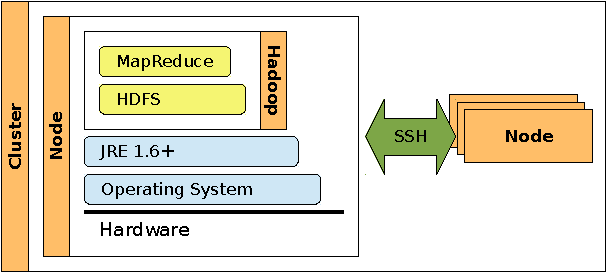
\includegraphics[width=0.7\textwidth]{imagenes/015.pdf}
 \caption{Hadoop over HDFS}
\label{fig:hadoopmapredhdfs}
\end{center}
\end{figure}

\begin{figure}[tbp]
\begin{center}
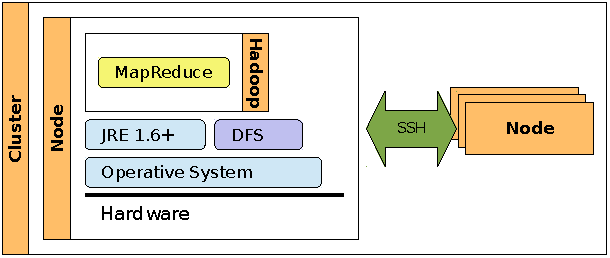
\includegraphics[width=0.7\textwidth]{imagenes/016.pdf}
 \caption{Hadoop over another DFS}
\label{fig:hadoopmapreddfs}
\end{center}
\end{figure}

As exposed in the figures, Hadoop runs atop a \emph{Java Virtual Machine} (\emph{JVM}) and inter-node communication is securely conveyed through \emph{SSH} tunnels. Besides, every Hadoop module includes a web server (\emph{Jetty}) to ease collecting and reporting status information with standard tools like web browsers or text processing CLI applications.

\section{Hadoop Distributed File System}\label{sec:hdfs}
\noindent HDFS has been designed to act as archival repository for huge masses of data whose main access pattern be \emph{write-one} \emph{read-many}. While it is no requisite for a data query to follow this access pattern, HDFS performance shines with read queries in batches. The underlying infrastructure, again, is composed by commodity machines that HDFS will manage to transform into a reliable, scalable, fault tolerant, self-balancing and network traffic-reducing data store. Yet, as individual nodes may be regular computers, in HDFS converge some operating limitations:

\begin{itemize}
 \item High \emph{data access time}. HDFS prioritizes large reads in batches and thus, reading small files is  discouraged. However, HDFS delivers \emph{very} high throughput by leveraging parallel reads on the cluster.
 \item High \emph{data write time} on many small files. Writing a file changes a block. Every file that be smaller than the HDFS block size must be persisted in a single block. That changed block must be sent out across the network to keep the file system coherently updated. Thus, appending to \emph{n} files may at least require updating \emph{n} blocks that would need be synchronized over the network.
 \item Multiple writers to the same file or \emph{not-append} file operations are not supported. HDFS is not a \emph{POSIX}-compilant file system as it implements only the set of operations required to maximize data throughput in distributed environments.
\end{itemize}

To organize storage HDFS takes from traditional file systems the concept of \emph{block}. In this case, an HDFS block is an abstraction atop the particular local file system with a double purpose:

\begin{description}
 \item[Lower DFS complexity:] Writing a block comprises storing the block data and meta-data, and handling information on how to locate the block on disk. Using the block as the minimum organizational structure simplifies the algorithms to manipulate de file system.
 \item[Increment flexibility:] files are free to grow over the size of an HDFS block with no penalty on access time or throughput.
\end{description}

To lay blocks in position, HDFS makes use of two processes: the \emph{DataNode} and the \emph{NameNode}. Besides, as support, from Hadoop 0.21.0 onward it is permitted the optional deploying of a \emph{Backup Node} and a \emph{Checkpoint Node} in the same cluster.

\subsection{Node Roles}\label{subsec:rolesnodos}
\noindent Figure \ref{fig:desplieguehdfs} shows a layered down HDFS deployment. In dotted line appear both the Backup Node and the Checkpoint Node.

\begin{figure}[tbp]
\begin{center}
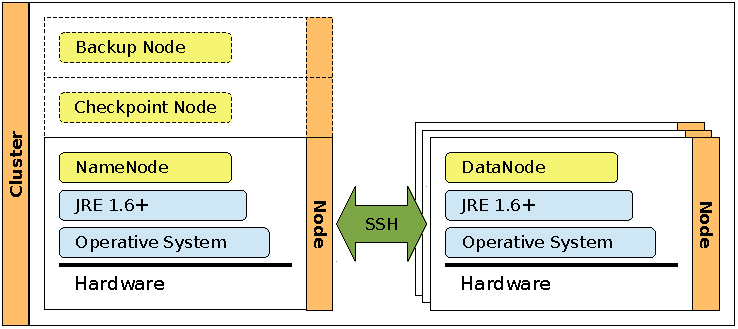
\includegraphics[width=0.9\textwidth]{imagenes/017.pdf}
 \caption{Typical HDFS deployment}
\label{fig:desplieguehdfs}
\end{center}
\end{figure}

\subsubsection{DataNode}\label{subsubsec:datanode}
\noindent DataNodes are those processes within nodes that handle the storage of HDFS blocks in their local drives. Every time a write to a file in a block succeeds, the DataNode in charge of the operation signals its supervising NameNode so that it can keep track the modifications to the DFS as they happen.

\subsubsection{NameNode}\label{subsubsec:namenode}
\noindent The NameNode is the process appointed to deal with the name space of the cluster. It has to handle the file system tree and meta-data that make possible recovering data from the DFS. It is such an important process that if it went down, every piece of data in HDFS would get lost, rendering impossible to match files with their container blocks. Therefore, the NameNode is seldom deployed with no Checkpoint Nodes or Backup Nodes when no other backup policity were implemented.

The information about the file system, the meta-data, is persisted to the NameNode both in-memory and disk. In this latter form, the meta-data is managed in two files: one contains the name space of the file system as an image (\texttt{fsimage}), the other progressively appends the changes to the fsimage (\emph{edits}) as a log. When the NameNode starts, it compiles an fsimage afresh by merging the existing fsimage with the edits file. As soon as changes to the HDFS are reported from the DataNodes, the NameNode will update the edits log but without touching the fsimage. In a typical secured deployment, the edits file is kept in-memory and in the local file system in the NameNode computer, and remotely via NFS.

\subsubsection{Checkpoint Node}\label{subsubsec:checkpointnode}
\noindent The Checkpoint Node is the means by which failure in the NameNode poses a smaller threat to the integrity of the data within HDFS. The idea behind the Checkpoint Node is to maintain a separate copy of the edits file so that it could periodically merge the fsimage with the edits, generating an updated fsimage to be uploaded to the NameNode. It should be noted that the Checkpoint Node does not listen to the network to record the modifications to the DFS in the edits file, it fetches the copy held by the NameNode itself. When the merging process be finished, the NameNode will be submitted the newly created fsimage, clearing out the old copy and reseting the edits file.

\subsubsection{Backup Node}\label{subsubsec:backupnode}
\noindent The Backup Node provides the same functionality as the Checkpoint Node by periodically creating restoration points of the name space but through a different approach. In this case, the Backup Node will download the fsimage file from the \emph{backed up} NameNode when booted, just like the Checkpoint Node, but it will receive notifications from the DataNodes on each modification to the HDFS, and will manage itself the merging between the fsimage and the edits file, effectively creating a new fsimage; the same behavior as the NameNode.

Compared to the Checkpoint Node this process draws less bandwidth due to the fact that it does not require to download the fsimage nor the edits file from the NameNode in order to stay synchronized.

The Hadoop version used in the VM of the solution, as will be described in section \ref{cap:solucion}, allows only a Backup Node per NameNode or multiple Checkpoint Nodes, not both. It should be noted that including a Backup Node in a cluster gives the possibility to run the NameNode with no persistent storage, i.e. with no allocated space in the local drive to write the fsimage and the edits file, making the Backup Node the sole responsible for the duty.

\subsection{Network Topology}\label{subsec:topologiared}
\noindent One of the fundamental parts to a file system in a distributed environment is the capacity to provide a transparent mechanism by which information is persisted securely while, at the same time, a certain amount of performance is maintained. HDFS makes use of an already discussed technique, \emph{replication}, that provides high performance, scalability and fault tolerance. Besides, HDFS has been designed to reduce the network congestion that stems from regular operation, giving special emphasis to the way in which data is to be distributed in the cluster, controlling replica count or distance between replicas, among other variables, to concrete the block allocation policy.

\subsubsection{Node Distance}\label{subsubsec:distnodos}
\noindent To support the features that have been mentioned, it is fundamental for the NameNode to possess some information on the participating DataNodes physical location. With that information, the NameNode would be able to balance the \emph{physical distance} of the replicas, bearing in mind that, as a general rule, fault tolerance increases with replica distance but the bandwidth available to transfer replicas narrows. Thus, the NameNode will have to distribute the replicas across the cluster with a procedure that kept the data in the cluster safe without clogging the network.

To effectively calculate the physical distance between two replicas, the NameNode will use an approximate measure of the physical distance of the nodes storing the replicas. Therefore, the problem lies in finding a formula to calculate the distance between any two nodes in the cluster.

IP-based networks arrange participating nodes in an abstract tree structure. In properly configured networks, the closer two nodes are physically the smaller the distance between their respective routing gateways. This idea, along with the fact that IP networks are tree-shaped, may be used recursively until the \emph{same} routing gateway was reached up from the initial nodes. So, the actual distance between two replicas is \emph{the number of steps required to find a common routing gateway, starting from the two nodes that stored the replicas}. The example below will clarify the procedure.

Only using the distance among replicas to distribute them lacks an important feature that would render the cluster failure-prone. In order to keep HDFS fault tolerant, the NameNode has to deal with halting nodes, clogged networks, etc. If a stalled node were the gateway to a set of nodes, e.g the nodes in the same rack, then the access to any replica within that cluster would be impossible, and worse, if every replica of an individual block were stored in this rack, the block would be inaccessible for the duration of the outage in the gateway. Therefore, a complementary mechanism should be devised to solve this distributing problems.

HDFS overcomes this limitations by mapping every IP address to a tuple with as many components as levels there were in the network --- typically \emph{three-tuples} \emph{(data center, rack, node)}. Figure \ref{fig:distnodos} shows the most common values of the replica distance. With the help of the figure the procedure to get to $d=4$ will be succinctly explained.

The upper left node holds the original block and the one pointed by the $d=4$-labeled edge a replica. Both blocks are stored in nodes within the same data center but in different racks, thus, their nearest common gateway would be the one managing the routing between those two racks. Besides, every rack has an internal gateway that must be traversed in order for the internal traffic to exit the rack. So, each node would have to take \emph{2 steps} to get to their common gateway --- from node to \emph{in-rack} gateway to \emph{off-rack} gateway --- coming to \emph{4 steps}.

\begin{figure}[tbp]
\begin{center}
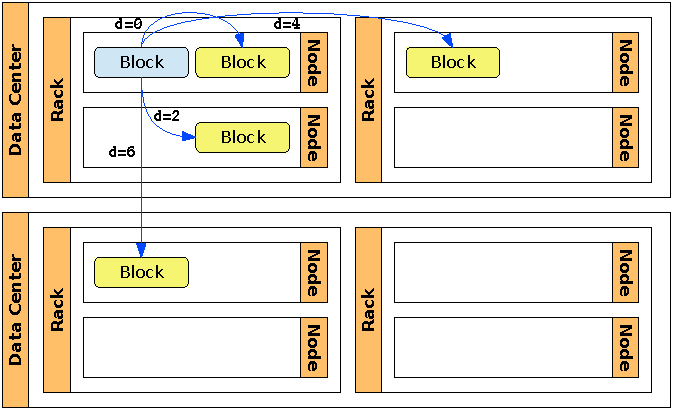
\includegraphics[width=0.85\textwidth]{imagenes/018.pdf}
 \caption{Replica distance}
\label{fig:distnodos}
\end{center}
\end{figure}

\subsubsection{Replication}\label{subsubsec:replicacionbloques}
\noindent Replication is a NameNode-controlled technique that relies on knowing the network topology to structure hierarchically the nodes in the cluster. Together with replica distance the NameNode is capable of enforcing a policy that balances data safety and throughput. What follows is the description of the method to distribute replicas over the cluster.

When a new block is written to HDFS --- or when an existing one is appended new data --- a predefined number of replicas have to be made and distributed. By default, the NameNode will maintain updated three replicas of each block. The first block is placed in a node at random prioritizing those not too full nor too busy. Then, the first replica is stored in the same node as the original block. The second replica is sent off-rack to a node at random, and finally, the third replica is stored in the same rack as the second replica but in a different node. If the \emph{replica factor} --- the total number of replicas every block will have --- were made higher, the successive replicas would be placed, again, in the same rack as the second one but in different nodes whenever possible.

This method provides the desirable equilibrium between fault tolerance --- by assuring two copies of a block exist in different racks ---, consumed bandwidth --- writing a new block would only need replicas to go through a single gateway as subsequent replicas are made within the rack ---, read performance --- making it possible for every read request to be fulfilled from nodes in two racks --- and balanced data distribution by executing the process just described. Figure \ref{fig:repbloque} exemplifies a factor 3 replication. The number in brackets indicates the order in which the replicas were created. The original block is in the upper left corner of the figure.

\begin{figure}[tbp]
\begin{center}
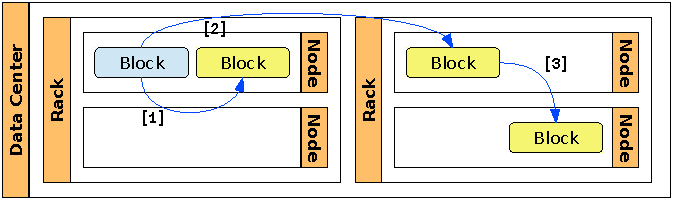
\includegraphics[width=0.85\textwidth]{imagenes/019.pdf}
 \caption{Replication factor 3}
\label{fig:repbloque}
\end{center}
\end{figure}


\section{Hadoop MapReduce}\label{sec:hadoopmapred}
\noindent In a typical Hadoop deployment, the execution layer is lied over HDFS. This execution module is basically an implementation of the ideas exposed in the Google paper on MapReduce \cite{googlemapreduce}. The core ideas that have been discussed for HDFS also hold true in this section, but with a different approach. Hadoop MapReduce architecture is also based on the Master-Worker model and so there appear two roles: a Master and a Worker.

The Master role is functionally covered by a process called the \emph{JobTracker}, whose main responsibility is task scheduling to workers. Complementarily, the Worker role is implemented in the \emph{TaskTracker} which will actually execute the individual tasks reporting their progress back to the JobTracker.

\subsection{Node Roles}\label{subsec:rolesnodosmapred}
\noindent Figure \ref{fig:desplieguehadoopmapred} shows the JobTracker and the TaskTracker in context, using HDFS as file system. To give a full picture, the HDFS processes, NameNode and DataNode, would have to be included.

\begin{figure}[tbp]
\begin{center}
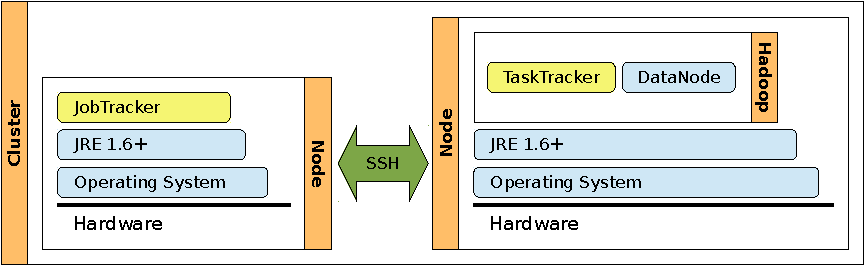
\includegraphics[width=0.9\textwidth]{imagenes/020.pdf}
 \caption{Hadoop MapReduce with HDFS}
\label{fig:desplieguehadoopmapred}
\end{center}
\end{figure}

Just as with HDFS, the JobTracker and the TaskTacker will be subsequently dissected.

\subsubsection{JobTracker}\label{subsubsec:jobtracker}
\noindent The JobTracker behaves in a very similar manner to the NameNode, but in this case it handles the scheduling part of job execution. A regular workflow starts with a client submitting both the algorithm and data to the cluster. The client is then returned an identification for the new job. The Jobtracker, when it had determined that the job should start, would initialize the job sending out to the TaskTrackers the code required to complete the execution. The TaskTrackers would be sent, each, a subset of the work to be completed for the job: a task in MapReduce nomenclature.

Distributing the work among TaskTrackers is done following the principle of maximum locality, i.e. making TaskTrackers process the parts of the job that refer to data stored closer to them. Enforcing this policy limits the amount of traffic flowing over the network and, at the same time, shortens data access time.

Running in an environment prone to error, the JobTracker must define a method to deal with a myriad of failures with limited impact on job throughput. To that end, the JobTracker maintains a list detailing task status. This list is updated by the JobTracker process continually polling the TaskTrackers for new information on the tasks. If a TaskTracker were to stop responding after multiple tries, the JobTracker would mark the task \emph{failed} to reschedule its execution at a later time.

More difficult to deal with would be the failure of the JobTracker process. The initial approach as proposed by Google in their paper \cite{googlemapreduce} is to discard unfinished jobs and try to reboot the service in an \emph{idle node} --- and online duty-free node ---, as only one JobTracker per cluster was supported. In Hadoop ecosystem \emph{Zookeeper} provides the means for running multiple instances of JobTrackers within the same cluster.

\subsubsection{TaskTracker}\label{subsubsec:tasktracker}
\noindent The TaskTracker is the process that executes MapReduce algorithms on data ideally stored in the node running the process. The TaskTracker will periodically communicate with the JobTracker to report status updates. As it has been discussed above, a failing TaskTracker will be unable to repeatedly \emph{pong} the JobTracker's \emph{ping}, effectively rendering the task inaccessible and due to be rescheduled to an idle TaskTracker.
